\chapter{Introducción}

\section{Consideraciones iniciales}

El marco de trabajo que se presenta en este libro parte de una cultura de solución de problemas adaptativa que apoya el desarrollo de productos y servicios, posibilitando la búsqueda de mejores formas de aprender y crear valor en ambientes laborales más cálidos y humanos. Al inicio del libro se relata el “qué” y el “porqué” de este marco, para luego pasar a contar el “cómo”, a un alto nivel y, desde esta perspectiva, ofrecer diferentes herramientas y prácticas que sirvan para ayudar a implementarlo y complementarlo con éxito.

\subsection{Definición}

Scrum es un marco de trabajo (framework) para construir y mantener productos complejos \cite{SBOK-2013} \cite{Scrum-Alliance-2015}. 
Scrum funciona como una implementación del ciclo de mejora continua de Deming (PDCA) y como una implementación de los principios ágiles y principios Scrum. Hay que tener en cuenta que Scrum no es exactamente un proceso íntegro, metodología completa o una técnica para construir productos; sino que, es un marco de trabajo dentro del cual se pueden emplear varias técnicas y procesos \cite{Agile-Atlas-2012}. En otras palabras, Scrum es un marco de trabajo que permite organizar a un equipo para que logre cierta cadencia, que es un ritmo sostenible y cíclico de trabajo a través de múltiples iteraciones de trabajo, en el transcurso de un ciclo de vida de un proyecto, en el que el equipo se siente cómodo entregando productos parciales y de valor para el cliente.

\subsection{Sobre si es una Metodología}

Hay quienes consideran que Scrum no es una metodología, entre otras cosas porque no especifica exactamente el cómo se hacen las cosas, 
sino que dice el qué hacer. Sin embargo, hay autores y guías que tratan a Scrum como metodología (por ejemplo la guía SBOK \footnote{\cite{SBOK-2013}, SCRUMstudy (2015).}, la ScrumAlliance \footnote{"Scrum is the leading agile development methodology", Learn About Scrum, Scrumalliance.org, 2015.} y Jeff Sutherland\footnote{\cite{Jeff-Sutherland-2016}}). De hecho en el informe original de Ken Schwaber se habla de metodología \cite{Ken-Schwaber-1995}. En consecuencia, se puede encontrar en numerosa bibliografía que el marco de trabajo Scrum puede ser denominado Metodología de Desarrollo Scrum o Metodología de Gestión de Proyectos Scrum. 
En el primer caso puede deberse a que se puede considerar una metodología como un proceso de desarrollo iterativo e incremental de productos \cite{Ken-Schwaber-1995}. Y en el segundo caso porque se puede considerar que es una alternativa a la gestión clásica de proyectos propuesta en marcos de trabajo como la guía de Gestión de Proyectos PMI. En este último sentido podemos recordar la definición original de Ken Schwaber: "Scrum es una metodología de gestión, mejora y mantenimiento de un sistema existente o prototipo de producción" \cite{Ken-Schwaber-1995}.
 
Por otro lado, considerando que Scrum define roles, artefactos, actividades, flujo del ciclo de actividades Scrum\footnote{\cite{Agile-Atlas-2012}}, reglas y algunas sugerencias de implementación como, además, al definir el flujo del ciclo de Scrum o flujo de trabajo, define parcialmente un cómo, en el cual se incluye una secuencia básica de cosas que hacer; por eso, y sin ser puristas, se puede considerar en forma práctica como una forma de metodología de trabajo y de gestión. O sea que puede funcionar como una metodología a alto nivel o plataforma de trabajo sobre la cual pueden funcionar otras metodologías, más específicas de producción y desarrollo, y otras técnicas y procesos. Por este motivo, puede ser adaptado a diversas empresas y organizaciones que trabajen con metodologías diferentes pero compatibles con los lineamientos de Scrum (sus valores y principios) y del Movimiento Ágil (enfoque ágil). Se puede usar Scrum y a su vez utilizar técnicas de otras metodologías para implementar sus actividades y sugerencias. O sea que cuando se usa este marco se hace una aproximación empleando diversas técnicas y, posiblemente, otras metodologías. Por eso, es recomendable que se lo denomine "marco de trabajo".

\subsection{Ámbito de aplicación}

Relacionado a su ámbito de aplicación, podemos analizar nuestro equipo o nuestra organización bajo el modelo Cynefin\footnote{Cynefin: Snowden (1999), "Liberating Knowledge"; Snowden (2003). "The new dynamics of strategy: Sense-making in a complex and complicated world"}. Con Cynefin podemos evaluar los múltiples factores en nuestro entorno y nuestra experiencia y determinar bajo qué dominio nos encontramos. Pues, Scrum no es un marco de trabajo orientado a implementarse en cualquier dominio y contexto. Scrum está pensado especialmente para proyectos bajo "dominios complejos" [Snowden 2007] (ver fig. \ref{fig:MarcoCynefinModel}) donde existe un grado alto de incertidumbre y baja predictibilidad y para sistemas adaptativos complejos, donde mismas causas pueden generar diferentes consecuencias o diferentes causas pueden generar mismas consecuencias. O sea que es útil en ámbitos con requisitos inciertos y riesgos técnicos altos. Nos permite encontrar prácticas emergentes en dominios complejos, como por ejemplo en la gestión de proyectos de innovación \cite{Martin-Alaimo-2014} y desarrollo de productos con requisito inciertos y cambiantes. Es decir, está orientado a contextos que necesitan niveles altos de creatividad, innovación, interacción y comunicación. Por este motivo, es bastante empleado en la industria de software, ya que en la misma existen contextos específicos de alta complejidad e incertidumbre con necesidad de creatividad e innovación. Pero también se utiliza en otras industrias con dominios de problemas de complejidad semejante. Por ejemplo ha sido empleado en: educación, organizaciones de campañas publicitarias, industria de productos de innovación, empresas de editoriales de libros, etcétera.

\begin{figure}[h]
  \centering
  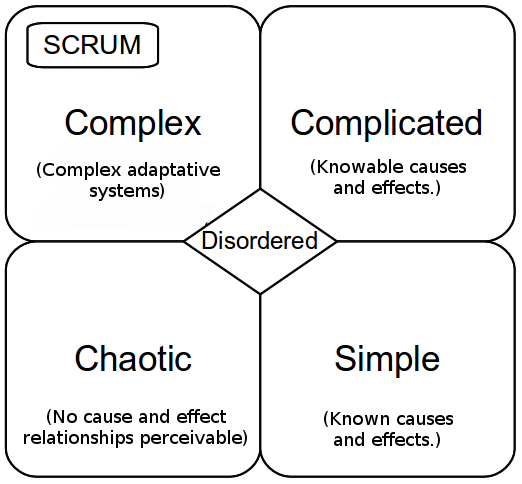
\includegraphics[width=0.50\textwidth]{MarcoCynefinModel}
  \caption{Scrum en el Modelo Cynefin}
  \centering
  \label{fig:MarcoCynefinModel} %\ref{fig:MarcoCynefinModel}
\end{figure}

\subsection{Visión general}

En esta metodología se definen los principios y valores a seguir, los roles, relaciones y responsabilidades, los artefactos o entidades manejadas en el proceso de trabajo y un conjunto de reuniones o actividades en un flujo de trabajo. Como resumen podemos ver la imagen de la figura \ref{fig:ScrumMapMind}.

\begin{figure}[h]
  \centering
  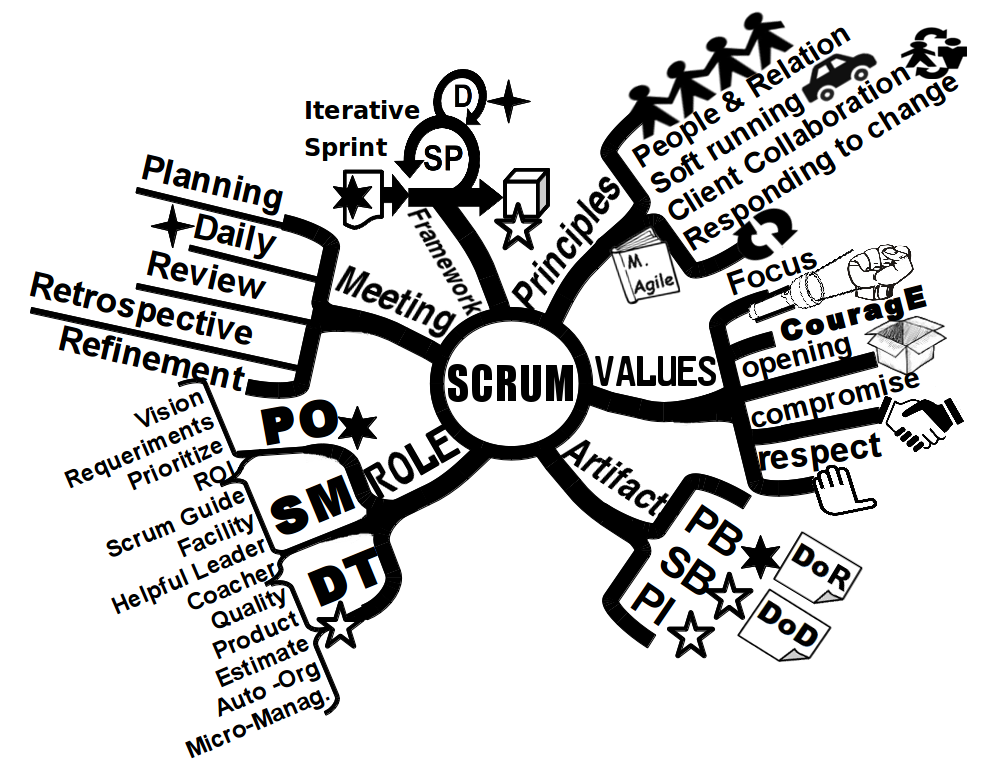
\includegraphics[width=0.99\textwidth]{ScrumMapMind}
  \caption{Mapa mental sobre Scrum}
  \centering
  \label{fig:ScrumMapMind} %\ref{fig:ScrumMapMind}
\end{figure}

En los siguientes capítulos se explicarán los diferentes aspectos y características de la propuesta de este marco de trabajo y al final, tras leer el libro, el mapa mental de la figura \ref{fig:ScrumMapMind} quedará explicado y será fácilmente entendible. 
